\documentclass[aspectratio=169,11pt]{beamer}

\usepackage[T1]{fontenc}
\usepackage[utf8]{inputenc}
\usepackage[brazilian]{babel}
\usepackage{lmodern}
\usepackage{graphicx}
\usepackage{booktabs}
\usepackage{hyperref}
\usepackage{multicol}
\usepackage{tikz}
\usepackage{amsmath}
\usepackage{array}

% -----------------------------------------------------------------------------
% Identidade visual
% -----------------------------------------------------------------------------
\definecolor{RoxoPrincipal}{HTML}{4D4057}
\definecolor{RoxoSecundario}{HTML}{75657F}
\definecolor{MalvaDestaque}{HTML}{9A6F86}
\definecolor{LavandaClaro}{HTML}{F1EDF3}
\definecolor{LavandaLinha}{HTML}{D8CFDD}
\definecolor{CinzaTexto}{HTML}{413C43}

\usetheme{default}
\useinnertheme{rounded}
\setbeamertemplate{navigation symbols}{}

\setbeamercolor{normal text}{fg=CinzaTexto,bg=white}
\setbeamercolor{structure}{fg=RoxoPrincipal}
\setbeamercolor{title}{fg=white}
\setbeamercolor{subtitle}{fg=white}
\setbeamercolor{author}{fg=white}
\setbeamercolor{institute}{fg=white!90}
\setbeamercolor{date}{fg=white!80}
\setbeamercolor{frametitle}{fg=white,bg=RoxoPrincipal}
\setbeamercolor{block title}{fg=white,bg=RoxoSecundario}
\setbeamercolor{block body}{fg=CinzaTexto,bg=LavandaClaro}
\setbeamercolor{block title alerted}{fg=white,bg=MalvaDestaque}
\setbeamercolor{block body alerted}{fg=CinzaTexto,bg=LavandaClaro}
\setbeamercolor{alerted text}{fg=MalvaDestaque}
\setbeamercolor{footline}{fg=RoxoPrincipal,bg=white}
\setbeamercolor{footline line}{bg=LavandaLinha}

\setbeamerfont{title}{size=\LARGE,series=\bfseries}
\setbeamerfont{subtitle}{size=\large}
\setbeamerfont{frametitle}{size=\large,series=\bfseries}
\setbeamerfont{footline}{size=\scriptsize}

% Logo da UFPE com uma base clara para contraste.
\newcommand{\marcaInstitucional}[1]{%
  \begin{tikzpicture}[baseline=(marca.base)]
    \node[fill=white,rounded corners=2pt,inner sep=2.2pt] (marca) {%
      
\includegraphics[height=#1]{imgs/logo_ufpe.png}%
    };
  \end{tikzpicture}%
}

% Cabeçalho roxo com a marca institucional em todos os slides de conteúdo.
\setbeamertemplate{frametitle}{%
  \nointerlineskip
  \begin{beamercolorbox}[
    wd=\paperwidth,ht=3.4ex,dp=1.45ex,leftskip=0.58cm,rightskip=1.75cm
  ]{frametitle}%
    \usebeamerfont{frametitle}\insertframetitle
  \end{beamercolorbox}%
  \begin{tikzpicture}[remember picture,overlay]
    \node[anchor=north east,fill=white,rounded corners=2pt,inner sep=1.2pt]
      at ([xshift=-0.32cm,yshift=-0.16cm]current page.north east)
      {
\includegraphics[height=0.52cm]{imgs/logo_ufpe.png}};
  \end{tikzpicture}%
}

% Rodapé leve, com seção atual e paginação em formato de cápsula.
\setbeamertemplate{footline}{%
  \leavevmode%
  \vbox{%
    \begin{beamercolorbox}[wd=\paperwidth,ht=0.22ex,dp=0ex]{footline line}
    \end{beamercolorbox}%
    \hbox{%
      \begin{beamercolorbox}[wd=.28\paperwidth,ht=3.0ex,dp=1.15ex,leftskip=0.55cm]{footline}
        \usebeamerfont{footline}\insertshortauthor
      \end{beamercolorbox}%
      \begin{beamercolorbox}[wd=.52\paperwidth,ht=3.0ex,dp=1.15ex,center]{footline}
        \usebeamerfont{footline}\insertsectionhead
      \end{beamercolorbox}%
      \begin{beamercolorbox}[wd=.20\paperwidth,ht=3.0ex,dp=0.65ex,rightskip=0.45cm plus 1fil]{footline}
        \tikz[baseline=-0.65ex]{%
          \node[fill=RoxoPrincipal,text=white,rounded corners=5pt,
            inner xsep=7pt,inner ysep=2.3pt] {%
            \usebeamerfont{footline}\insertframenumber\,/\,\inserttotalframenumber
          };
        }%
      \end{beamercolorbox}%
    }%
  }%
  \vskip0pt%
}

% -----------------------------------------------------------------------------
% Informações editáveis da apresentação
% -----------------------------------------------------------------------------
\newcommand{\telefone}{(81) 98538-4702}
\newcommand{\email}{Romadeoliveira@hotmail.com}
\newcommand{\linkedin}{linkedin.com/in/romariojonas-veloso-427373175}
\newcommand{\portfolio}{romariojonas.com}
\newcommand{\lattes}{lattes.cnpq.br/7040983804231610}


% Campos explicitamente reservados para dados ainda não coletados.
\newcommand{\aguardando}{\textcolor{MalvaDestaque}{\scriptsize A preencher}}
\newcommand{\campoimagem}[2]{%
  \begin{center}
  \begin{tikzpicture}
    \draw[draw=LavandaLinha,dashed,thick,fill=LavandaClaro,rounded corners=4pt]
      (0,0) rectangle (10.6,3.45);
    \node[align=center,text=RoxoSecundario] at (5.3,1.72)
      {\large #1\\[4pt]\scriptsize Inserir registro após a prática};
  \end{tikzpicture}\par
  \vspace{0.08cm}
  {\scriptsize\itshape #2}
  \end{center}}
\newcommand{\campoimagemdois}[2]{%
  \begin{center}
  \begin{tikzpicture}
  \draw[draw=LavandaLinha,dashed,fill=LavandaClaro,rounded corners=4pt]
    (0,0) rectangle (5.0,2.65);
  \node[align=center,text=RoxoSecundario] at (2.5,1.32)
    {\small #1\\[4pt]\tiny A inserir após o laboratório};
  \end{tikzpicture}\par
  {\scriptsize\itshape #2}
  \end{center}}

\title[6ª Prática -- Circuitos 2]{6ª Prática de Laboratório}
\subtitle{Amplificador emissor comum: análise teórica, parâmetros $g$ e validação experimental}
\author[Romário Jonas O. Veloso]{Romário Jonas O. Veloso}
\institute{Engenharia Eletrônica -- Universidade Federal de Pernambuco\\
Centro de Tecnologia e Geociências -- CTG\\
Departamento de Eletrônica e Sistemas -- DES\\
Disciplina: EL216 -- Circuitos 2}
\date{16 de novembro de 2026}

\begin{document}

% ===== INÍCIO: slides/01_capa.tex =====
% Capa
{
\setbeamercolor{background canvas}{bg=RoxoPrincipal}
\setbeamertemplate{footline}{}
\begin{frame}[plain]
  \begin{center}
    \vspace{0.25cm}
    \marcaInstitucional{1.55cm}\par
    \vspace{0.45cm}
    {\usebeamerfont{title}\color{white}\inserttitle\par}
    \vspace{0.22cm}
    {\usebeamerfont{subtitle}\color{white!82}\insertsubtitle\par}
    \vspace{0.48cm}
    {\color{MalvaDestaque}\rule{0.22\textwidth}{2pt}}\par
    \vspace{0.48cm}
    {\usebeamerfont{author}\color{white}\insertauthor\par}
    \vspace{0.12cm}
    {\usebeamerfont{institute}\color{white!84}\insertinstitute\par}
    \vfill
    {\color{white!72}\small \insertdate\quad\textbullet\quad Recife -- Pernambuco}
  \end{center}
\end{frame}
}
% ===== FIM: slides/01_capa.tex =====


% ===== INÍCIO: slides/02_sumario.tex =====
% Sumário
\begin{frame}{Sumário}
  \tableofcontents
\end{frame}
% ===== FIM: slides/02_sumario.tex =====


\section{Introdução}

% ===== INÍCIO: slides/03_contexto.tex =====

\begin{frame}{Contexto}
  \begin{block}{6ª Prática -- EL216 / Circuitos 2}
  Estudo de um amplificador com transistor bipolar NPN na configuração
  \textbf{emissor comum}, utilizando polarização por realimentação
  do coletor para a base. \cite{cabral2022pratica6}
  \end{block}
  \begin{itemize}
    \item Modelo de grandes sinais: obtenção do ponto de operação DC.
    \item Modelo de pequenos sinais: transcondutância e resistência $r_\pi$.
    \item Quadripolo: determinação analítica e experimental dos parâmetros $g$.
    \item Comparação entre teoria, simulação e medições em bancada.
  \end{itemize}
  \vspace{0.15cm}
  {\scriptsize Fonte: Cabral (2022), roteiro da prática e material de aula.}
\end{frame}
% ===== FIM: slides/03_contexto.tex =====


% ===== INÍCIO: slides/04_circuito.tex =====

\begin{frame}{Circuito sob estudo}
  \begin{columns}[c,onlytextwidth]
    \begin{column}{0.62\textwidth}
    \centering
    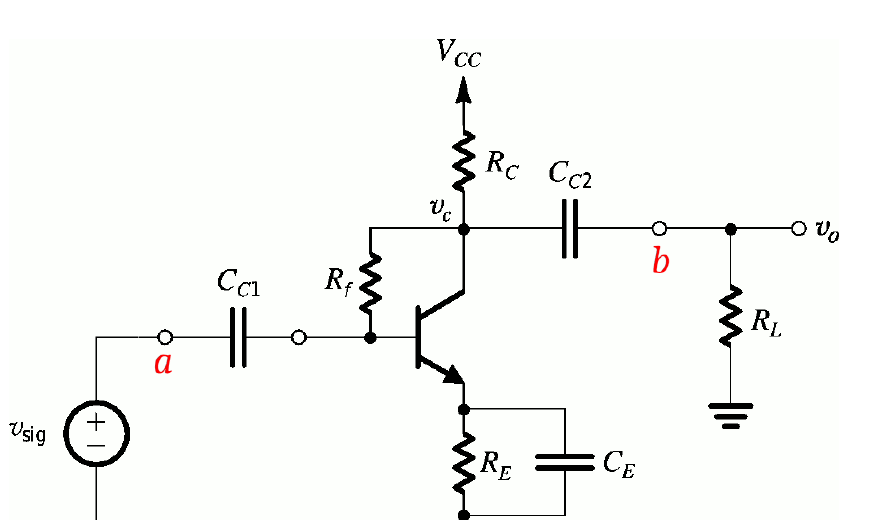
\includegraphics[width=\linewidth,height=0.68\textheight,keepaspectratio]{imgs/circuito_roteiro.png}
    \par{\scriptsize Figura 1 -- Esquema do amplificador emissor comum.\par
    Fonte: Cabral (2022), 6ª Prática, p. 2.}
    \end{column}
    \begin{column}{0.36\textwidth}
    \begin{block}{Topologia}
    \small
    \begin{itemize}
      \item $R_C$: carga de coletor.
      \item $R_f$: realimentação DC/AC.
      \item $R_E$: estabilidade da polarização.
      \item $C_{C1}$ e $C_{C2}$: acoplamento.
      \item $C_E$: desvio de $R_E$ em AC.
    \end{itemize}
    \end{block}
    \end{column}
  \end{columns}
\end{frame}
% ===== FIM: slides/04_circuito.tex =====


\section{Objetivos}

% ===== INÍCIO: slides/05_objetivos.tex =====

\begin{frame}{Objetivos}
  \begin{block}{Objetivo geral}
  Determinar os parâmetros $g$ de um amplificador emissor comum e
  confrontar a descrição linear com medições de entrada e saída.
  \end{block}
  \begin{enumerate}
    \item Calcular as correntes e tensões de polarização do transistor.
    \item Obter $g_m$, $r_\pi$ e as equações de pequenos sinais.
    \item Deduzir $g_{11}$, $g_{12}$, $g_{21}$ e $g_{22}$ por análise nodal.
    \item Estudar $V_2$, $I_1$, $R_{in}$ e $A_v$ em função de $R_L$.
    \item Estimar os parâmetros $g$ a partir das medições, via MMEQ.
  \end{enumerate}
\end{frame}
% ===== FIM: slides/05_objetivos.tex =====


\section{Metodologia}

% ===== INÍCIO: slides/06_dados.tex =====

\begin{frame}{Dados do roteiro e materiais}
  \begin{columns}[T,onlytextwidth]
    \begin{column}{0.52\textwidth}
      \centering\small
      \begin{tabular}{ll}
        \toprule
        \textbf{Grandeza} & \textbf{Valor}\tabularnewline
        \midrule
        $V_{CC}$ & $12\,\mathrm{V}$\\
        $R_C$ & $4{,}7\,\mathrm{k}\Omega$\\
        $R_E$ & $470\,\Omega$\\
        $R_f$ & $150\,\mathrm{k}\Omega$\\
        $C_{C1}=C_{C2}=C_E$ & $10\,\mu\mathrm{F}$\\
        $f$ & $5\,\mathrm{kHz}$\\
        $\beta$; $V_{BE0}$ & $150$; $0{,}7\,\mathrm{V}$\\
        $R_L$ & $680$ a $50\,680\,\Omega$\\
        \bottomrule
      \end{tabular}
    \end{column}
    \begin{column}{0.44\textwidth}
      \begin{block}{Instrumentação}
        \small
        Fonte DC, gerador de sinais, osciloscópio, multímetro,
        protoboard e simulador LTspice.
      \end{block}
      \begin{block}{Medições adicionais}
      \small
       $R_{m1}=220\,\Omega$ e $R_{m2}=680\,\Omega$;
       potenciômetro de $50\,\mathrm{k}\Omega$ no procedimento completo.
      \end{block}
    \end{column}
  \end{columns}
  \vspace{0.2cm}
  {\scriptsize Fonte: Cabral (2022), p. 6--8.}
\end{frame}
% ===== FIM: slides/06_dados.tex =====


% ===== INÍCIO: slides/07_procedimento.tex =====

\begin{frame}{Etapas do trabalho}
  \begin{columns}[T,onlytextwidth]
    \begin{column}{0.32\textwidth}
      \begin{block}{1. Análise teórica}
        \small Polarização DC, modelo híbrido-$\pi$, parâmetros $g$ e
        previsões em função da carga.
      \end{block}
    \end{column}
    \begin{column}{0.32\textwidth}
      \begin{block}{2. Simulação}
        \small LTspice: ponto de operação e formas de onda para $5$ kHz.
      \end{block}
    \end{column}
    \begin{column}{0.32\textwidth}
      \begin{block}{3. Bancada}
        \small Medição das portas e estimação dos parâmetros por mínimos quadrados.
      \end{block}
    \end{column}
  \end{columns}
  \vspace{0.45cm}
  \begin{alertblock}{Situação atual}
    \small Etapa teórica desenvolvida. Fotos de montagem,
    capturas da simulação e valores experimentais serão inseridos após sua obtenção.
  \end{alertblock}
\end{frame}
% ===== FIM: slides/07_procedimento.tex =====


\section{Análise teórica: grandes sinais}

% ===== INÍCIO: slides/08_modelo_dc.tex =====

\begin{frame}{Grandes sinais -- modelo DC}
  \begin{columns}[T,onlytextwidth]
    \begin{column}{0.54\textwidth}
      \begin{block}{Hipóteses}
        \begin{itemize}\small
          \item Capacitores em circuito aberto.
          \item A fonte de sinal não altera a polarização DC.
          \item $I_C=\beta I_B$, $I_E=I_C+I_B$.
          \item $V_{BE0}\approx0{,}7\,\mathrm{V}$.
        \end{itemize}
      \end{block}
    \end{column}
    \begin{column}{0.44\textwidth}
      \begin{block}{Relações fundamentais}
        \[
        I_C=\beta I_B
        \]
        \[
        I_E=(\beta+1)I_B
        \]
        \[
        I_{R_C}=I_E,\quad I_{R_f}=I_B
        \]
      \end{block}
    \end{column}
  \end{columns}
  \vspace{0.2cm}
  \centering\small A polarização deve manter $V_C>V_B>V_E$ para operação na região ativa direta.
\end{frame}
% ===== FIM: slides/08_modelo_dc.tex =====


% ===== INÍCIO: slides/09_correntes_dc.tex =====

\begin{frame}{Grandes sinais -- determinação das correntes}
  \small
  Pela LKT na malha $V_{CC}\!\to\!R_C\!\to\!R_f\!\to\!V_{BE0}\!\to\!R_E$:
  \[
    V_{CC} - R_C I_E - R_f I_B - V_{BE0} - R_E I_E=0
  \]
  Substituindo $I_E=(\beta+1)I_B$ e isolando $I_B$:
  \[
  \boxed{I_B=\frac{V_{CC}-V_{BE0}}{R_f+(\beta+1)(R_C+R_E)}}
  \]
  \[
  I_B=\frac{12-0{,}7}{150\,000+151(4\,700+470)}
  =\boxed{12{,}142\,\mu\mathrm A}
  \]
  \[
  I_C=\beta I_B=\boxed{1{,}82127\,\mathrm{mA}}\qquad
  I_E=(\beta+1)I_B=\boxed{1{,}83341\,\mathrm{mA}}
  \]
\end{frame}
% ===== FIM: slides/09_correntes_dc.tex =====


% ===== INÍCIO: slides/10_tensoes_dc.tex =====

\begin{frame}{Grandes sinais -- tensões e ponto de operação}
  \begin{columns}[T,onlytextwidth]
    \begin{column}{0.55\textwidth}
      \small
      \[
      V_E=R_E I_E=\boxed{0{,}86170\,\mathrm V}
      \]
      \[
      V_B=V_E+V_{BE0}=\boxed{1{,}56170\,\mathrm V}
      \]
      \[
      V_C=V_{CC}-R_C I_E=\boxed{3{,}38297\,\mathrm V}
      \]
      \[
      V_{CE}=V_C-V_E=\boxed{2{,}52127\,\mathrm V}
      \]
    \end{column}
    \begin{column}{0.42\textwidth}
      \begin{block}{Verificação}
        \[
        V_{BE}=0{,}700\,\mathrm V
        \]
        \[
        V_{CB}=V_C-V_B
        \]
        \[
        V_{CB}=1{,}82127\,\mathrm V>0
        \]
        \centering\small Região ativa direta, no modelo adotado.
      \end{block}
    \end{column}
  \end{columns}
  \vspace{0.18cm}
  \centering{\scriptsize Resultados calculados com $\beta=150$ e componentes nominais do roteiro.}
\end{frame}
% ===== FIM: slides/10_tensoes_dc.tex =====


\section{Análise teórica: pequenos sinais}

% ===== INÍCIO: slides/11_modelo_ac.tex =====

\begin{frame}{Pequenos sinais -- modelo equivalente}
  \begin{columns}[c,onlytextwidth]
    \begin{column}{0.61\textwidth}
      \centering
      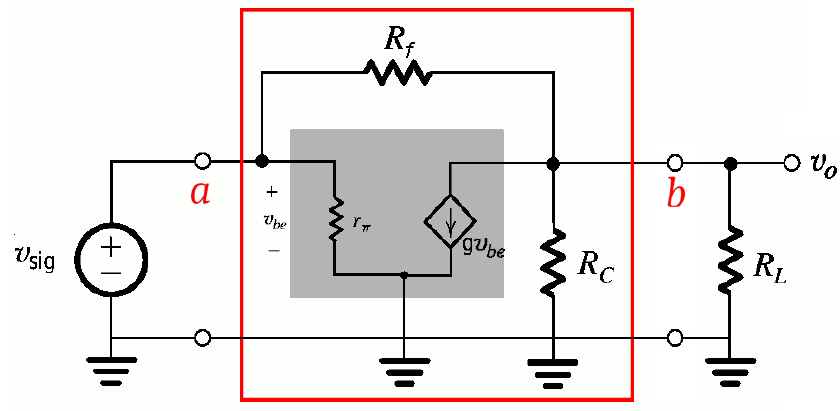
\includegraphics[width=\linewidth,height=0.61\textheight,keepaspectratio]{imgs/modelo_pequenos_sinais.png}
      \par{\scriptsize Figura 2 -- Modelo de pequenos sinais e limites do quadripolo.\par
      Fonte: Cabral (2022), roteiro de aula, slide 8.}
    \end{column}
    \begin{column}{0.36\textwidth}
      \begin{block}{Aproximações}
        \small
        \begin{itemize}
          \item Capacitores em curto para AC.
          \item Fonte $V_{CC}$ em terra AC.
          \item $C_E$ desvia $R_E$.
          \item $v_{be}=V_1$.
          \item $i_c=g_m v_{be}$.
        \end{itemize}
      \end{block}
    \end{column}
  \end{columns}
\end{frame}
% ===== FIM: slides/11_modelo_ac.tex =====


% ===== INÍCIO: slides/12_parametros_transistor.tex =====

\begin{frame}{Pequenos sinais -- parâmetros do transistor}
  \begin{columns}[T,onlytextwidth]
  \begin{column}{0.51\textwidth}
    \begin{block}{Transcondutância}
    \[
      g_m=30I_C
    \]
    \[
      g_m=30(1{,}82127\times10^{-3})
    \]
    \[
      \boxed{g_m=54{,}6381\,\mathrm{mS}}
    \]
    \end{block}
  \end{column}
  \begin{column}{0.46\textwidth}
    \begin{block}{Resistência dinâmica de entrada}
    \[
      r_\pi=\frac{\beta}{g_m}
    \]
    \[
      r_\pi=\frac{150}{0{,}0546381}
    \]
    \[
      \boxed{r_\pi=2{,}74534\,\mathrm{k}\Omega}
    \]
    \end{block}
  \end{column}
  \end{columns}
  \vspace{0.24cm}
  \centering\small Modelo linear: $i_c=g_mv_{be}$ e $i_b=v_{be}/r_\pi$.
\end{frame}
% ===== FIM: slides/12_parametros_transistor.tex =====


\section{Quadripolo e parâmetros g}

% ===== INÍCIO: slides/13_quadripolo.tex =====

\begin{frame}{Quadripolo -- formulação e equações nodais}
  \small
  Definição dos parâmetros de admitância inversa (parâmetros $g$):
  \[
  \begin{bmatrix} I_1\\ V_2\end{bmatrix}=
  \begin{bmatrix} g_{11}&g_{12}\\g_{21}&g_{22}\end{bmatrix}
  \begin{bmatrix} V_1\\I_2\end{bmatrix}
  \]
  \begin{block}{Nó da base (porta 1)}
  \[
  \boxed{I_1=\left(\frac{1}{r_\pi}+\frac{1}{R_f}\right)V_1-\frac{V_2}{R_f}}
  \]
  \end{block}
  \begin{block}{Nó do coletor (porta 2)}
  \[
  \boxed{I_2=\left(g_m-\frac{1}{R_f}\right)V_1+\left(\frac{1}{R_C}+\frac{1}{R_f}\right)V_2}
  \]
  \end{block}
\end{frame}
% ===== FIM: slides/13_quadripolo.tex =====


% ===== INÍCIO: slides/14_deducao_parametros.tex =====

\begin{frame}{Parâmetros $g$ -- solução algébrica}
  \small
  Isolando $V_2$ na segunda equação nodal:
  \[
  V_2=\underbrace{\frac{R_C(1-g_mR_f)}{R_C+R_f}}_{g_{21}}V_1
  +\underbrace{\frac{R_CR_f}{R_C+R_f}}_{g_{22}}I_2
  \]
  Substituindo em $I_1$ e agrupando os coeficientes:
  \[
  I_1=\underbrace{\left[\frac{1}{r_\pi}+\frac{1+g_mR_C}{R_C+R_f}\right]}_{g_{11}}V_1
  +\underbrace{\left[-\frac{R_C}{R_C+R_f}\right]}_{g_{12}}I_2
  \]
  \begin{block}{Sinais e unidades}
  \scriptsize Correntes $I_1$ e $I_2$ positivas entrando no quadripolo.
  $g_{11}$ em S; $g_{22}$ em $\Omega$; $g_{12}$ e $g_{21}$ adimensionais.
  \end{block}
\end{frame}
% ===== FIM: slides/14_deducao_parametros.tex =====


% ===== INÍCIO: slides/15_matriz_numerica.tex =====

\begin{frame}{Parâmetros $g$ -- resultados numéricos}
  \[
  \boxed{\mathbf G=
  \begin{bmatrix}
  2{,}03070\,\mathrm{mS} & -0{,}0303814\\
  -248{,}967 & 4{,}55721\,\mathrm{k}\Omega
  \end{bmatrix}}
  \]
  \vspace{0.25cm}
  \begin{columns}[T,onlytextwidth]
  \begin{column}{0.48\textwidth}
  \begin{block}{Equação da porta 1}
  \small
  \[
  I_1=g_{11}V_1+g_{12}I_2
  \]
  \end{block}
  \end{column}
  \begin{column}{0.48\textwidth}
  \begin{block}{Equação da porta 2}
  \small
  \[
  V_2=g_{21}V_1+g_{22}I_2
  \]
  \end{block}
  \end{column}
  \end{columns}
  \vspace{0.3cm}
  \centering\scriptsize Parâmetros calculados para os elementos nominais e $\beta=150$.
\end{frame}
% ===== FIM: slides/15_matriz_numerica.tex =====


\section{Previsões teóricas}

% ===== INÍCIO: slides/16_ganho_rin.tex =====

\begin{frame}{Tensão de saída e resistência de entrada}
  \small
  Para uma carga $R_L$, a corrente de saída definida entrando no quadripolo é:
  \[
  I_2=-\frac{V_2}{R_L}
  \]
  Assim, de $V_2=g_{21}V_1+g_{22}I_2$:
  \[
  \boxed{A_v=\frac{V_2}{V_1}=\frac{g_{21}R_L}{R_L+g_{22}}}
  \]
  Substituindo em $I_1=g_{11}V_1+g_{12}I_2$:
  \[
  \boxed{R_{in}=\frac{V_1}{I_1}=\left(g_{11}-\frac{g_{12}A_v}{R_L}\right)^{-1}}
  \]
  \vspace{0.15cm}
  \centering\scriptsize $V_2=A_vV_1$ e $I_1=V_1/R_{in}$ para cada carga.
\end{frame}
% ===== FIM: slides/16_ganho_rin.tex =====


% ===== INÍCIO: slides/17_resultados_cargas.tex =====

\begin{frame}{Previsões para as cargas solicitadas}
  \small
  Com $V_1=30\,\mathrm{mV}$ de \textbf{pico} (caso teórico do roteiro):
  \vspace{0.3cm}
  \centering
  \begin{tabular}{lrr}
  \toprule
  \textbf{Grandeza} & $R_L=680\,\Omega$ & $R_L=50\,680\,\Omega$\\
  \midrule
  $A_v$ & $-32{,}326$ & $-228{,}426$\\
  $R_{in}$ & $1{,}705\,\mathrm{k}\Omega$ & $0{,}528\,\mathrm{k}\Omega$\\
  $V_2$ (pico, algébrico) & $-0{,}970\,\mathrm{V}$ & $-6{,}853\,\mathrm{V}$\\
  $I_1$ (pico) & $17{,}593\,\mu\mathrm A$ & $56{,}813\,\mu\mathrm A$\\
  \bottomrule
  \end{tabular}
  \vspace{0.32cm}
  \begin{alertblock}{Limite do modelo linear}
  \small O resultado na carga elevada é extrapolação de pequenos sinais:
  a excursão negativa disponível no coletor pode causar saturação e distorção.
  Na bancada, o roteiro pede $V_1=30\,\mathrm{mV_{pp}}$, que equivale a $15\,\mathrm{mV}$ de pico.
  \end{alertblock}
\end{frame}
% ===== FIM: slides/17_resultados_cargas.tex =====


% ===== INÍCIO: slides/18_curvas_ganho.tex =====

\begin{frame}{Curvas teóricas -- ganho e resistência de entrada}
  \begin{columns}[c,onlytextwidth]
    \begin{column}{0.49\textwidth}
      \centering
      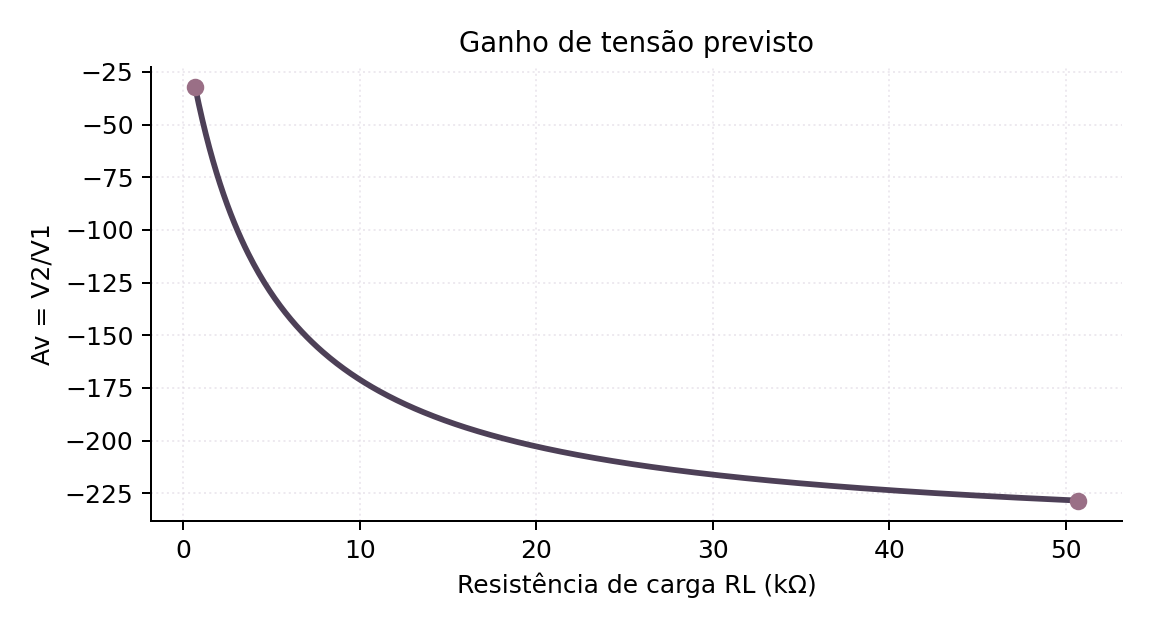
\includegraphics[width=\linewidth]{imgs/curva_ganho.png}
      {\scriptsize (a) $A_v$ em função de $R_L$.}
    \end{column}
    \begin{column}{0.49\textwidth}
      \centering
      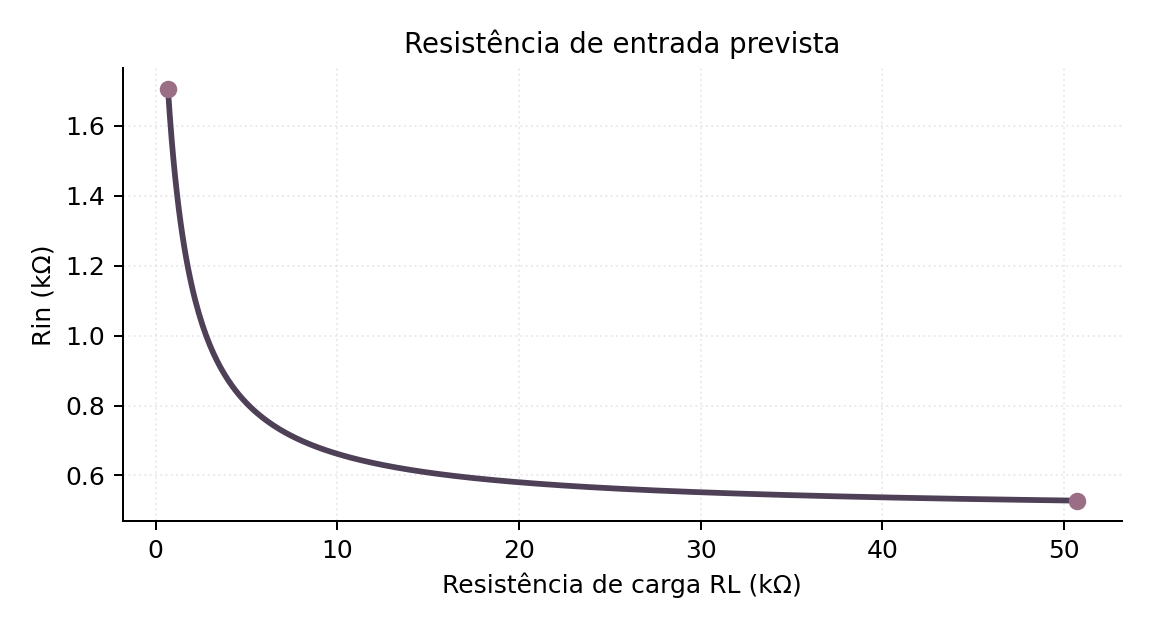
\includegraphics[width=\linewidth]{imgs/curva_rin.png}
      {\scriptsize (b) $R_{in}$ em função de $R_L$.}
    \end{column}
  \end{columns}
  \vspace{0.25cm}
  \centering\scriptsize Figura 3 -- Previsões obtidas a partir dos parâmetros $g$.
  Fonte: cálculos teóricos, elaboração própria.
\end{frame}
% ===== FIM: slides/18_curvas_ganho.tex =====


% ===== INÍCIO: slides/19_curvas_sinais.tex =====

\begin{frame}{Curvas teóricas -- tensão e corrente de entrada}
  \begin{columns}[c,onlytextwidth]
    \begin{column}{0.49\textwidth}
      \centering
      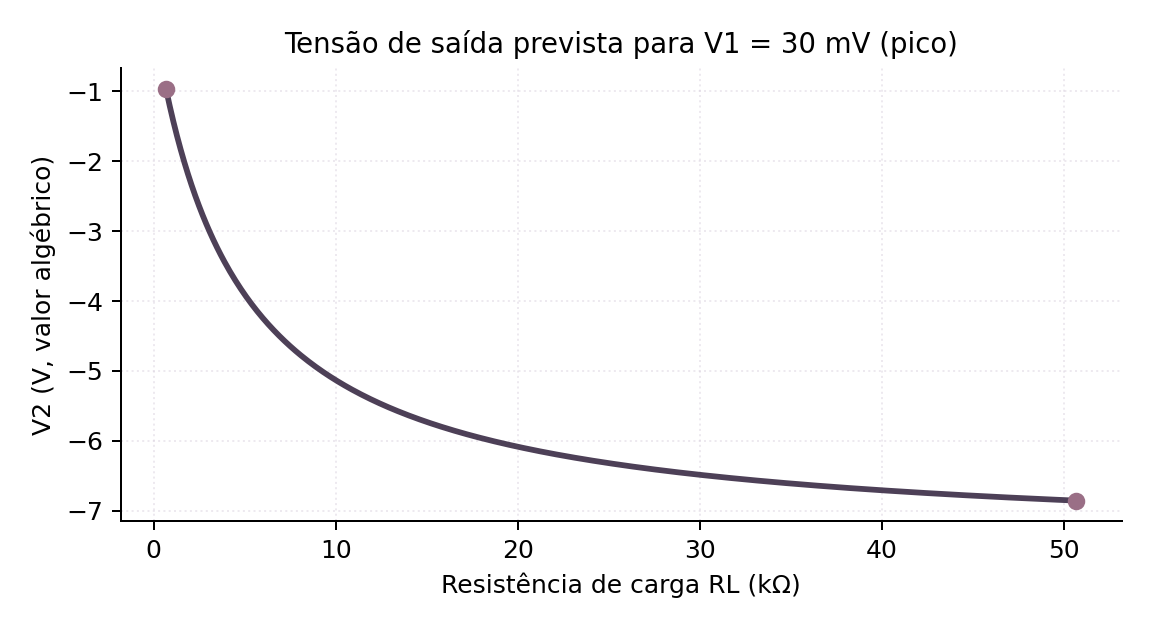
\includegraphics[width=\linewidth]{imgs/curva_v2.png}
      {\scriptsize (a) $V_2$ para $V_1=30\,\mathrm{mV}$ de pico.}
    \end{column}
    \begin{column}{0.49\textwidth}
      \centering
      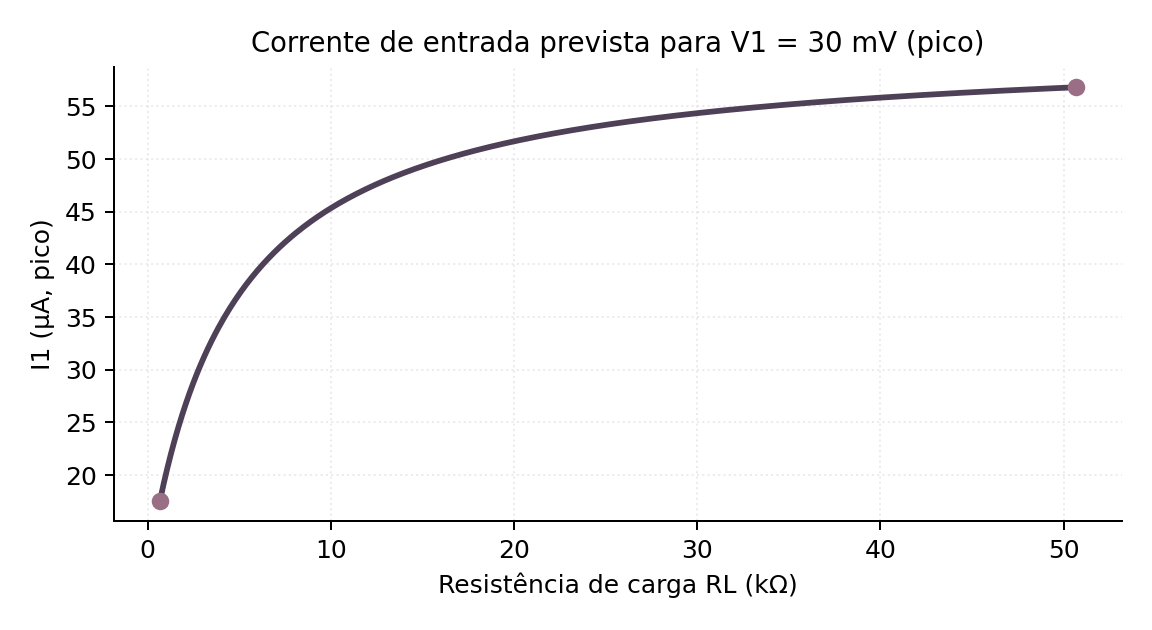
\includegraphics[width=\linewidth]{imgs/curva_i1.png}
      {\scriptsize (b) $I_1$ para $V_1=30\,\mathrm{mV}$ de pico.}
    \end{column}
  \end{columns}
  \vspace{0.25cm}
  \centering\scriptsize Figura 4 -- Previsões lineares em função de $R_L$.
  Valores de saída elevados podem não ser realizáveis sem distorção.
\end{frame}
% ===== FIM: slides/19_curvas_sinais.tex =====


\section{Simulação e laboratório}

% ===== INÍCIO: slides/20_simulacao.tex =====

\begin{frame}{Simulação -- configuração no LTspice}
  \begin{columns}[T,onlytextwidth]
  \begin{column}{0.48\textwidth}
    \begin{block}{Ponto de operação DC}
      \ttfamily\small .op
    \end{block}
    \begin{block}{Sinal de entrada}
      \normalfont\small $f=5\,\mathrm{kHz}$, onda senoidal;
      ajustar a amplitude para obter $V_1=30\,\mathrm{mV_{pp}}$.
    \end{block}
  \end{column}
  \begin{column}{0.48\textwidth}
    \begin{block}{Análise no tempo}
      \ttfamily\small .tran 5m
    \end{block}
    \begin{block}{Grandezas de interesse}
      \normalfont\small $V_B$, $V_C$, $V_E$, $I_C$, $I_E$,
      formas de onda $V_1(t)$, $V_2(t)$ e ganho experimental.
    \end{block}
  \end{column}
  \end{columns}
  \vspace{0.23cm}
  \begin{alertblock}{Variante montada sem potenciômetro}
    \small Com $R_L=680\,\Omega$, obtém-se um único ponto da curva. Para reproduzir
    as variações de carga do roteiro, será necessário alterar $R_L$ ou empregar o potenciômetro.
  \end{alertblock}
\end{frame}
% ===== FIM: slides/20_simulacao.tex =====


% ===== INÍCIO: slides/21_registros_simulacao.tex =====

\begin{frame}{Registros da simulação -- a inserir}
  \begin{columns}[T,onlytextwidth]
  \begin{column}{0.49\textwidth}
    \campoimagemdois{Esquema no LTspice}{Figura 5 -- Circuito implementado no simulador.}
  \end{column}
  \begin{column}{0.49\textwidth}
    \campoimagemdois{Formas de onda $V_1$ e $V_2$}{Figura 6 -- Tensões de entrada e saída em $5$ kHz.}
  \end{column}
  \end{columns}
  \vspace{0.22cm}
  \begin{block}{Resultados numéricos da simulação}
    \small $V_1=\,$\aguardando \quad
    $V_2=\,$\aguardando \quad
    $A_v=\,$\aguardando
  \end{block}
\end{frame}
% ===== FIM: slides/21_registros_simulacao.tex =====


% ===== INÍCIO: slides/22_montagem.tex =====

\begin{frame}{Montagem experimental -- registro fotográfico}
  \campoimagem{Foto do circuito na protoboard}{Figura 7 -- Montagem do amplificador emissor comum com transistor 2N3904.}
  \vspace{-0.05cm}
  \centering\scriptsize Conferir pinagem C/B/E e polaridade dos capacitores antes da alimentação.
\end{frame}
% ===== FIM: slides/22_montagem.tex =====


% ===== INÍCIO: slides/23_medicoes_dc.tex =====

\begin{frame}{Medições em bancada -- polarização DC}
  \small
  Fonte estabilizada ligada; gerador de sinais desligado. Registrar os valores
  com referência ao terra do circuito.\par
  \vspace{0.23cm}
  \begin{center}
  \begin{tabular}{lcc}
    \toprule
    \textbf{Grandeza} & \textbf{Previsão teórica} & \textbf{Valor medido}\\
    \midrule
    $V_B$ & $1{,}56170\,\mathrm{V}$ & \aguardando\\
    $V_C$ & $3{,}38297\,\mathrm{V}$ & \aguardando\\
    $V_E$ & $0{,}86170\,\mathrm{V}$ & \aguardando\\
    $I_C$ & $1{,}82127\,\mathrm{mA}$ & \aguardando\\
    $I_E$ & $1{,}83341\,\mathrm{mA}$ & \aguardando\\
    \bottomrule
  \end{tabular}\par
  \vspace{0.20cm}
  {\scriptsize Tabela 1 -- Ponto de operação: cálculo teórico versus medição experimental.}
  \end{center}
\end{frame}
% ===== FIM: slides/23_medicoes_dc.tex =====


% ===== INÍCIO: slides/24_medicoes_ac.tex =====

\begin{frame}{Medições em bancada -- pequenas variações AC}
  \begin{columns}[T,onlytextwidth]
  \begin{column}{0.49\textwidth}
    \campoimagemdois{Osciloscópio}{Figura 8 -- Registro de $V_1(t)$ e $V_2(t)$.}
  \end{column}
  \begin{column}{0.49\textwidth}
    \small
    \begin{tabular}{ll}
      \toprule
      \textbf{Registro} & \textbf{Resultado}\\
      \midrule
      $V_1$ & \aguardando\\
      $V_2$ & \aguardando\\
      $V_{m1}$ & \aguardando\\
      $V_{m2}$ & \aguardando\\
      $R_L$ & \aguardando\\
      \bottomrule
    \end{tabular}
    \vspace{0.12cm}
    \par{\scriptsize Tabela 2 -- Medição para uma carga selecionada.}
  \end{column}
  \end{columns}
  \vspace{0.20cm}
  \begin{block}{Variação de carga no roteiro}
    \small Medir nas posições mínima e máxima e nos níveis $0{,}2$;
    $0{,}3$; $0{,}4$; $0{,}5$; $0{,}6$; $0{,}7$; $0{,}8$; $0{,}9$ de $V_{2,\max}$.
    \textcolor{MalvaDestaque}{\textit{Tabela completa: a preencher após as medições.}}
  \end{block}
\end{frame}
% ===== FIM: slides/24_medicoes_ac.tex =====


% ===== INÍCIO: slides/24b_serie_medicoes.tex =====

\begin{frame}{Medições em função da carga -- tabela de coleta}
  \scriptsize
  Registrar as amplitudes com $5\,\mathrm{kHz}$ e $V_1=30\,\mathrm{mV_{pp}}$.
  \vspace{0.14cm}\par
  \begin{center}
    \renewcommand{\arraystretch}{1.09}
    \begin{tabular}{lccccc}
      \toprule
      \textbf{Condição} & $R_L$ ($\Omega$) & $V_1$ & $V_2$ & $V_{m1}$ & $V_{m2}$\\
      \midrule
      Pot. máximo  & -- & -- & -- & -- & --\\
      Pot. mínimo  & -- & -- & -- & -- & --\\
      $0{,}2V_{2,\max}$ & -- & -- & -- & -- & --\\
      $0{,}3V_{2,\max}$ & -- & -- & -- & -- & --\\
      $0{,}4V_{2,\max}$ & -- & -- & -- & -- & --\\
      $0{,}5V_{2,\max}$ & -- & -- & -- & -- & --\\
      $0{,}6V_{2,\max}$ & -- & -- & -- & -- & --\\
      $0{,}7V_{2,\max}$ & -- & -- & -- & -- & --\\
      $0{,}8V_{2,\max}$ & -- & -- & -- & -- & --\\
      $0{,}9V_{2,\max}$ & -- & -- & -- & -- & --\\
      \bottomrule
    \end{tabular}
    \vspace{0.10cm}\par
    {\scriptsize Tabela 3 -- Espaços reservados para a série de medições. ``--'' = a preencher.}
  \end{center}
  \vspace{-0.08cm}
  \begin{alertblock}{Atenção}
    \scriptsize A versão com $R_L=680\,\Omega$ fixo não permite completar esta tabela sem
    modificar a carga entre as medições.
  \end{alertblock}
\end{frame}
% ===== FIM: slides/24b_serie_medicoes.tex =====


% ===== INÍCIO: slides/25_mmeq.tex =====

\begin{frame}{Pós-laboratório -- estimação dos parâmetros $g$}
  \small
  Para cada uma das $N$ medições, relacionar as duas portas por:
  \[
    I_1^{(k)}=g_{11}V_1^{(k)}+g_{12}I_2^{(k)},\qquad
    V_2^{(k)}=g_{21}V_1^{(k)}+g_{22}I_2^{(k)}
  \]
  Formulação matricial do método dos mínimos erros quadráticos (MMEQ):
  \[
  \underbrace{\begin{bmatrix}V_1^{(1)}&I_2^{(1)}\\[-1pt]\vdots&\vdots\\V_1^{(N)}&I_2^{(N)}\end{bmatrix}}_{A}
  \underbrace{\begin{bmatrix}g_{11}&g_{21}\\g_{12}&g_{22}\end{bmatrix}}_{X}
  \approx
  \underbrace{\begin{bmatrix}I_1^{(1)}&V_2^{(1)}\\[-1pt]\vdots&\vdots\\I_1^{(N)}&V_2^{(N)}\end{bmatrix}}_{B}
  \]
  \[
    \boxed{\hat X=\underset{X}{\operatorname{argmin}}\,\|AX-B\|_F^2}
  \]
  \vspace{0.10cm}
  \centering\textcolor{MalvaDestaque}{\scriptsize Parâmetros $g$ estimados: a preencher após inserir as medições.}
\end{frame}
% ===== FIM: slides/25_mmeq.tex =====


% ===== INÍCIO: slides/25b_curvas_experimentais.tex =====

\begin{frame}{Pós-laboratório -- curvas de porta}
  \begin{columns}[c,onlytextwidth]
  \begin{column}{0.49\textwidth}
     \campoimagemdois{$V_2$ em função de $I_2$}{Figura 9 -- Curva prevista e pontos medidos.}
  \end{column}
  \begin{column}{0.49\textwidth}
     \campoimagemdois{$I_1$ em função de $I_2$}{Figura 10 -- Curva prevista e pontos medidos.}
  \end{column}
  \end{columns}
  \vspace{0.23cm}
  \begin{block}{Comparação}
    \small Inserir valores e curvas a partir da série de medições e
    confrontar com as equações obtidas para o quadripolo.
  \end{block}
\end{frame}
% ===== FIM: slides/25b_curvas_experimentais.tex =====


% ===== INÍCIO: slides/25c_curvas_experimentais.tex =====

\begin{frame}{Pós-laboratório -- ganho e resistência medidos}
  \begin{columns}[c,onlytextwidth]
  \begin{column}{0.49\textwidth}
     \campoimagemdois{$R_{in}$ em função de $R_L$}{Figura 11 -- Curva teórica e pontos medidos.}
  \end{column}
  \begin{column}{0.49\textwidth}
     \campoimagemdois{$A_v$ em função de $R_L$}{Figura 12 -- Curva teórica e pontos medidos.}
  \end{column}
  \end{columns}
  \vspace{0.22cm}
  \begin{block}{Cálculos experimentais}
    \small $I_1=V_{m1}/R_{m1}$; $I_2=-V_{m2}/R_{m2}$ (orientação indicada).\\
    $R_{in}=V_1/I_1$; $A_v=V_2/V_1$.
  \end{block}
\end{frame}
% ===== FIM: slides/25c_curvas_experimentais.tex =====


\section{Conclusões}

% ===== INÍCIO: slides/26_conclusao.tex =====

\begin{frame}{Considerações finais}
  \begin{itemize}
    \item Polarização teórica: $I_C=1{,}82127\,\mathrm{mA}$ e
      $V_{CE}=2{,}52127\,\mathrm V$, consistentes com a região ativa.
    \item Modelo de pequenos sinais: $g_m=54{,}6381\,\mathrm{mS}$ e
      $r_\pi=2{,}74534\,\mathrm{k}\Omega$.
    \item Os parâmetros $g$ permitem prever o ganho e a resistência de entrada
      para diferentes cargas.
    \item A validação em bancada e a estimação por MMEQ
      permanecem \textbf{pendentes de execução experimental}.
  \end{itemize}
  \begin{alertblock}{Completar após a prática}
    \small Inserir fotos, tensões/correntes medidas, comparação com LTspice,
    curvas experimentais e discussão das diferenças teoria--experimento.
  \end{alertblock}
\end{frame}
% ===== FIM: slides/26_conclusao.tex =====


\section{Referências}

% ===== INÍCIO: slides/27_referencias.tex =====

% Referências no formato BibTeX, com quebras automáticas se necessário.
{\setbeamertemplate{bibliography item}[text]
\setbeamercolor{bibliography item}{fg=MalvaDestaque}
\setbeamercolor{bibliography entry author}{fg=RoxoPrincipal}
\begin{frame}[allowframebreaks]{Referências bibliográficas}
  \scriptsize
  \nocite{*}
  \bibliographystyle{plain}
  \bibliography{referencias}
\end{frame}}
% ===== FIM: slides/27_referencias.tex =====



% ===== INÍCIO: slides/28_contracapa.tex =====

{
\setbeamercolor{background canvas}{bg=LavandaClaro}
\setbeamertemplate{footline}{}
\begin{frame}[plain]
  \begin{center}
    \vfill
    \marcaInstitucional{1.45cm}\par
    \vspace{0.32cm}
    {\color{RoxoPrincipal}\LARGE\bfseries 6ª Prática -- Circuitos 2}\par
    \vspace{0.22cm}
    {\large Amplificador emissor comum e parâmetros $g$}\par
    \vspace{0.50cm}
    {\color{MalvaDestaque}\rule{0.25\textwidth}{2pt}}\par
    \vspace{0.38cm}
    {\large Romário Jonas O. Veloso}\par
    {\small Universidade Federal de Pernambuco -- UFPE}\par
    {\scriptsize Recife, 16 de novembro de 2026}
    \vfill
  \end{center}
\end{frame}
}
% ===== FIM: slides/28_contracapa.tex =====


% ===== INÍCIO: slides/29_obrigado.tex =====

{
\setbeamercolor{background canvas}{bg=RoxoPrincipal}
\setbeamertemplate{footline}{}
\begin{frame}[plain]
  \begin{center}
    \vfill
    \marcaInstitucional{1.25cm}\par
    \vspace{0.45cm}
    {\color{white}\Huge\bfseries OBRIGADO}\par
    \vspace{0.35cm}
    {\color{MalvaDestaque}\rule{0.22\textwidth}{2pt}}\par
    \vspace{0.75cm}
    {\color{white}\Large Romário Jonas O. Veloso}\par
    \vspace{0.16cm}
    {\color{white!85}\small EL216 -- Circuitos 2}\par
    \vfill
  \end{center}
\end{frame}
}
% ===== FIM: slides/29_obrigado.tex =====

\end{document}
